\documentclass[11pt]{article}

\usepackage[english]{babel}
\usepackage[margin=0.8in]{geometry}

% Math/Greek packages
\usepackage{amssymb,amsmath,amsthm, mathtools} 
\usepackage{algorithm, algorithmic}
\usepackage{upgreek, siunitx}
\usepackage{setspace}

% Graphics/Presentation packages
\usepackage{multirow}
\usepackage{graphicx}
\usepackage{cancel}
\usepackage{tabulary, enumitem, array}
\usepackage{xparse,mleftright,tikz}
\usepackage{physics}

% Misc packages
\usepackage{fancyhdr}


\usepackage[export]{adjustbox}

\usepackage{esint}

\sisetup{locale=US,group-separator = {,}}
\usepackage[colorlinks=true, allcolors=blue]{hyperref}


% Box function - update this as more sophisticated solutions are found
\newcommand\mybox[2][]{\tikz[overlay]\node[fill=blue!20,inner sep=2pt, anchor=text, rectangle, rounded corners=1mm,#1] {#2};\phantom{#2}}
\renewcommand{\arraystretch}{1.2}

% General macro declarations


\makeatletter
\let\oldabs\abs
\def\abs{\@ifstar{\oldabs}{\oldabs*}}
%
\let\oldnorm\norm
\def\norm{\@ifstar{\oldnorm}{\oldnorm*}}
\makeatother

\begin{document}

\title{PHSX 462: HW02}
\author{William Jardee}
\maketitle

\section*{Question 1}
 Show that $\Psi = e^{ig}\Psi^\prime$ is a solution to 
\[\left[\frac{1}{2m}\left(-i\hbar \nabla - q \vec{A}\right)^2\right]\Psi = i \hbar \pdv{\Psi}{t}\]
 where 
\begin{align*}
g(\vec{r}) & = \frac{q}{h}\int_\mathcal{O}^{\vec{r}} \vec{A}(\vec{r}^\prime)\cdot \dd{\vec{r}} & -\frac{\hbar^2}{2m}\laplacian{\Psi^\prime} &= i \hbar \pdv{\Psi^\prime}{t}
\end{align*}

In the hints is also provided that $g = \frac{q}{\hbar} \alpha \eval^{\vec{r}}_{\mathcal{O}}$, since the $\curl{A} = 0$. So, $\grad{g} = \frac{q}{\hbar} A\eval^{\vec{r}}_{\mathcal{O}} = \frac{q}{\hbar}A(\vec{r})$. The only other thing that needs to be noticed is that $g$ is independent of $t$, thus it can be moved inside a partial derivative with respect to $t$.

\begin{flalign*}
\left[\frac{1}{2m}\left(-i\hbar \nabla - qA\right)^2\right]\Psi & = \left[\frac{1}{2m}\left(-i\hbar \nabla - qA\right)\left(-i\hbar \nabla - qA\right)\right]e^{ig}\Psi^\prime &\\
&= \frac{1}{2m}\left(-i\hbar \nabla -qA\right)\left[-i\hbar \left(\grad{e^{ig}}\right)\Psi^\prime - i\hbar e^{ig}\grad{\Psi^\prime} - qA e^{ig}\Psi^\prime\right]&\\
&= \frac{1}{2m}\left(-i\hbar \nabla -qA\right)\left[-i\hbar e^{ig}\left(\grad{ig}\right)\Psi^\prime - i\hbar e^{ig}\grad{\Psi^\prime} - qA e^{ig}\Psi^\prime\right]&\\
&= \frac{1}{2m}\left(-i\hbar \nabla -qA\right)\left[-i\hbar e^{ig}i\frac{q}{\hbar}A\Psi^\prime - i\hbar e^{ig}\grad{\Psi^\prime} -qA e^{ig}\psi^\prime\right]&\\
&= \frac{1}{2m}\left(-i\hbar \nabla -qA\right)\left[-i\hbar e^{ig}\grad{\Psi^\prime}\right]&\\
& = \frac{1}{2m}\left[\hbar e^{ig}i\grad{g}\grad{\Psi^\prime} - \hbar e^{ig}\laplacian{\Psi^\prime} + qAi\hbar e^{ig}\grad{\Psi^\prime}\right]&\\
& = \frac{1}{2m}\left[\hbar e^{ig}i\frac{q}{\hbar}A \grad{\Psi^\prime} - \hbar e^{ig}\laplacian{\Psi^\prime} + qAi\hbar e^{ig}\grad{\Psi^\prime}\right]&\\
& = -\frac{1}{2m}\hbar e^{ig}\laplacian{\Psi^\prime}&\\
& = -\frac{\hbar}{2m}e^{ig}\laplacian{\Psi^\prime} & \\
& = e^{ig}\pdv{\Psi^\prime}{t} = \pdv{e^{ig}\Psi^\prime}{t} = \pdv{\Psi}{t}
\end{flalign*}

 
%----------------------------------------------------------------------------
\newpage 

\section*{Griffiths 7.1}
Find the first-order correction to the allowed energies and the first three terms of the first order correction to the ground state, $\Psi_1^1$.
\[H^\prime = \alpha \delta(x - a/2)\]

Before we get started, let's remind ourselves of the general solutions to an infinite potential well:
\begin{align*}
E_n^0 & = \hbar^2 \frac{n^2 \pi^2}{2a^2 m} & \ket{\psi^0_m} & \rightarrow \sqrt{\frac{2}{a}}\sin(\frac{n \pi}{a}x)
\end{align*}

\begin{enumerate}[label=\alph*)]
\item 
\begin{flalign*}
E_n^1 &= \ev{H_1}{\Psi_n^0}&\\
& = \ev{\alpha \delta\left(x-\frac{a}{2}\right)}{\Psi_n^0}&\\
& = \alpha \frac{2}{a}\sin[2](\frac{n\pi}{a}\frac{a}{2})
\end{flalign*}

Using the properties of the $\sin$ function, if $n$ is even then $\sin(k \pi) = 0$ such that $k \in \mathbb{N}$. So, the even energies are not changed, but the odd ones are. This is a nature of what the probability distribution looks like. If the $n$ is odd, then a node is located at the center of the well and the delta function will not have an impact. 

\begin{equation*}
E_n^1  = \left\{
        \begin{array}{ll}
            \frac{2}{a} & \quad n \text{ is odd} \\
            0 & \quad n \text{ is even}
        \end{array}
    \right.
\end{equation*}

\item 
For this part we need to recall:
\[\ket{\Psi_n^1} = \sum_{m\neq n}\frac{\mel{\Psi_m^0}{H^\prime}{\Psi_n^0}}{E_n^0 - E_m^0}\ket{\Psi_m^0}\]

now, simply doing the calculation we get that:

\begin{flalign*}
\ket{\Psi_1^1} & = \sum_{m\neq 1}\frac{\mel{\Psi_m^0}{H^\prime}{\Psi_1^0}}{E_1^0 - E_m^0}\ket{\Psi_m^0}&\\
& = \sum_{m \neq 1} \frac{1}{E_1^0 - E_m^0}\frac{2}{a}\int \sin(\frac{n\pi}{a}x)\delta\left(x - \frac{a}{2}\right)\sin(\frac{\pi}{a}x)\dd{x}\ket{\Psi_m^0} &\\
& = \sum_{m \neq 1}\frac{1}{E_1^0 - E_m^0}\frac{2}{a} \sin(\frac{n\pi}{a}\frac{a}{2})\ket{\Psi_m^0}&\\
&= \sum_{m \neq 1}\frac{1}{E_1^0 - E_m^0}\frac{2}{a} \sin(\frac{n\pi}{2})\ket{\Psi_m^0}&\\
& = \frac{4ma}{\hbar^2 \pi^2}\left(\frac{1}{1-3^2}\sin(\frac{3\pi}{2})\sin(\frac{3\pi}{2}x) + \frac{1}{1-5^2}\sin(\frac{5\pi}{2})\sin(\frac{5\pi}{2}x) \right. \\
& \left. \qquad + \frac{1}{1-7^2}\sin(\frac{7\pi}{2})\sin(\frac{7\pi}{2}x) + \cdots\right)&\\
&=  \frac{4ma}{\hbar^2 \pi^2} \left(\frac{1}{8}\sin(\frac{3\pi}{2}x) -\frac{1}{24}\sin(\frac{5\pi}{2}x) + \frac{1}{48}\sin(\frac{7\pi}{2}x) + \cdots \right)
\end{flalign*}

So, the first three terms in the first order correction is: 
\[\boxed{\ket{\Psi_1^1} = \frac{4ma}{\hbar^2 \pi^2} \left(\frac{1}{8}\sin(\frac{3\pi}{2}x) -\frac{1}{24}\sin(\frac{5\pi}{2}x) + \frac{1}{48}\sin(\frac{7\pi}{2}x)\right)}\]

\end{enumerate}

%----------------------------------------------------------------------------
\newpage 

\section*{Griffiths 7.2}
Find the exact solution to the permutated system, then find the first-order perturbation in the energy and compare the two.
\[V(x) = \frac{1}{2}kx^2\, ; \, k \rightarrow (1+\varepsilon)k\]

\begin{enumerate}[label=\alph*)]
\item This part is pretty straight forward, so let's just do it.
\begin{flalign*}
E_n &= \left(n + \frac{1}{2}\right)\hbar \omega &\\
& = \left(n + \frac{1}{2}\right)\hbar \sqrt{\frac{k}{m}} &\\
& \rightarrow \left(n + \frac{1}{2}\right)\hbar \sqrt{\frac{(1+ \varepsilon)k}{m}} & \text{(Changing $k \rightarrow (1+\varepsilon)k$\,)}\\
& = \left(n + \frac{1}{2}\right)\hbar \sqrt{\frac{k}{m}}\sqrt{1+\varepsilon}&\\
& = \left[\left(n + \frac{1}{2}\right)\hbar \sqrt{\frac{k}{m}} \, \right]\left[1 + \frac{\varepsilon}{2} - \frac{\varepsilon^2}{8} + \frac{\varepsilon^3}{16} - \frac{5\varepsilon^4}{128} + \cdots\right] & \text{ (Assuming that $\varepsilon < 1$)} \\
& \rightarrow \left[\left(n + \frac{1}{2}\right)\hbar \sqrt{\frac{k}{m}} \, \right]\left[1 + \frac{\varepsilon}{2} - \frac{\varepsilon^2}{8}\right]&
\end{flalign*}

\item We are p
\begin{flalign*}
 E^\prime_n &= \ev{H^\prime}{\Psi_n^0} &\\
 & = \ev{\varepsilon\frac{1}{2}kx^2}{\Psi^0_n}&\\
 &= \varepsilon\ev{\frac{1}{2}kx^2}{\Psi^0_n} &\\
 & = \varepsilon \hbar \sqrt{\frac{k}{m}}\left(n + \frac{1}{2}\right)\braket{\Psi_n^0}{\Psi_n^0}
&\\
& = \varepsilon \sqrt{\frac{k}{m}}\left(n+\frac{1}{2}\right)
\end{flalign*}

We have to recognize that the permutation is on the potential energy, not the total energy. Using the Vivial Theorem to draw a parallel to the classical system: $E = \ev{V} + \ev{T}$ and $\ev{V} = \ev{T}$. So, $\ev{V} = \frac{1}{2}E$

Using this, the first order correction is: $\boxed{E_n^1 = \left[\sqrt{\frac{k}{m}}\left(n+\frac{1}{2}\right)\right]\frac{\varepsilon}{2}}$; which is exactly what we got for part {\bf a)}.

If it wasn't clear earlier:
\[\boxed{H^\prime_n = \varepsilon \frac{1}{2}kx^2}\]


\end{enumerate}


%----------------------------------------------------------------------------
\newpage 

\section*{Griffiths 7.4}
Find the exact energies of a permutated two-level system. Then take the second order expansion of $\lambda$ and set $\lambda=1$. Verify that this is consistent with the perturbation theory that we derived. When does this converge if $V_{aa} = V_{bb} = 0$
\begin{align*}
H^0 & = \mqty(E^0_a & 0 \\ 0  & E^0_b) & H^\prime & =  \lambda \mqty(V_{aa} & V_{ab} \\ V_{ba} & V_{bb})
\end{align*}
\[V_{ba} = V_{ab}^*\]

\begin{enumerate}[label=\alph*)]
\item 

\[H = H_0 + H_1 = \mqty[E_a^0 + \lambda v_{aa} & \lambda v_{ab} \\ \lambda v_{ba} & E_b^0 + \lambda v_{bb}] \rightarrow \mqty[A & \lambda v_{ab} \\ \lambda v^*_{ab} & B] \qquad \text{ s.t. } \mqty{A = E_a^0 + \lambda v_{aa} \\ B = E_b^0 + \lambda v_{bb}}\]

Looking for the eigenvalues of $H$
\begin{flalign*}
\mqty|A - E & \lambda v_{ab} \\ \lambda v^*_{ab} & B-E| & = AB - E(A+B) + E^2 + \lambda^2 \left|v_{ab}\right|^2 & \\
& = E^2 - E(A+B) + AB + C & \text{s.t. } C = \lambda^2 \left|v_{ab}\right|^2\\
\end{flalign*}
\begin{flalign*}
E & = \frac{(A+B)\pm \sqrt{(A+B)^2 - 4(AB+C)}}{2}&\\
& = \frac{(A+B)\pm \sqrt{(A-B)^2 - 4C}}{2} &\\
& = \frac{1}{2}\left[(A+B)\pm (A-B)\left(1 - \frac{4C}{2(A-B)^2} - \left(\frac{4C}{(A-B)^2}\right)^2 \frac{1}{8} + \cdots \right)\right] & \\
& \boxed{= \frac{1}{2}\left[(A+B) \pm \left((A-B) - \frac{2C}{A_B}\right) - \frac{2C^2}{(A-B)^3} + \cdots\right]}
\end{flalign*}
\item Assuming that $E_a^0 \, \& \, E_b^0 \gg \lambda v_{aa} \, \&\,  \lambda v_{bb} \longrightarrow [A-B] \approx [E_a^0 - E_b^0] $:
\begin{flalign*}
E & \approx \frac{1}{2}\left[(A+B)\pm \left((A-B) - \frac{2C}{E_a^0 -E_b^0}\right)\right]&\\
& = \frac{1}{2}\left[E_a^0 + E_b^0 + \lambda(v_{aa} + v_{bb}) \pm \left(E_a^0 - E_b^0 + \lambda(v_{aa} - v_{bb}) - \frac{2\lambda^2 \left|v_{ab}\right|^2}{E_a^0-E_b^0}\right)\right]&\\
& \rightarrow \frac{1}{2}\left[E_a^0 + E_b^0 + v_{aa} + v_{bb} \pm \left(E_a^0 - E_b^0 + v_{aa} - v_{bb} - \frac{2\left|v_{ab}\right|^2}{E_a^0-E_b^0}\right)\right] & \text{by setting } \lambda = 1
\end{flalign*}
\[\boxed{\mqty{E_+ = E_a^0+v_{aa} + \frac{\left|v_{ab}\right|^2}{E_b^0 - E_a^0} \\ E_- = E_b^0+v_{bb} + \frac{\left|v_{ab}\right|^2}{E_a^0 - E_b^0}}}\]

Checking this against our equation for the first order correction:
\begin{flalign*}
E^1 & = \ev{H^1}{+}&\\
&= \mqty[1 \\ 0]^T \mqty[v_{aa} & v_{ab} \\ v_{ab}^* & v_{bb}]\mqty[1 \\ 0] = \mqty[1 & 0]\mqty[v_{aa} \\ v_{ab}^*] = v_{aa}
\end{flalign*}
\begin{flalign*}
E^1 & = \ev{H^1}{-}&\\
&= \mqty[0 \\ 1]^T \mqty[v_{aa} & v_{ab} \\ v_{ab}^* & v_{bb}]\mqty[0 \\ 1] = \mqty[0 & 1]\mqty[v_{ab} \\ v_{bb}] = v_{bb}
\end{flalign*}
Bingo!

Now, checking for the second order:
\begin{flalign*}
E_a^2 & = \frac{\left|\mqty[1 & 0 ] \mqty[v_{aa} & v_{ab} \\ v_{ab}^* & v_{bb}]\right|^2}{E_- - E_+}&\\
&= \frac{\left|\mqty[1 & 0]\mqty[v_{ab} \\ v_{bb}]\right|^2}{E_a - E_b} = \frac{\left|v_{ab}\right|^2}{E_a-E_b} 
\end{flalign*}
And, by a symmetric calculation:\\
$E_b^2 = \frac{\left|v_{ab}\right|^2}{E_b - E_a}$\\
This is the same second order correction that we have! \checkmark

\item 
In the exact solution, we used the binomial expansion on $\sqrt{1 - \frac{4C}{(A-B)^2}}$. So, we need
\begin{flalign*}
1 & > \frac{4C}{(A-B)^2} = \frac{4\lambda^2\left|v_{ab}\right|^2}{(E_a^0 + \lambda v_{aa} - E_b^0 - \lambda v_{bb})^2} > \frac{4\lambda^2\left|v_{ab}\right|^2}{(E_a^0 - E_b^0)^2}&\\
\end{flalign*}
By setting $\lambda = 1$ and some algebra:
\[\boxed{\left|\frac{v_{ab}}{E_a^0 - E_b^0}\right|<\frac{1}{2}}\]

\end{enumerate}

%----------------------------------------------------------------------------
\newpage 

\section*{Question 5}

\begin{figure}[!ht]
\centering
	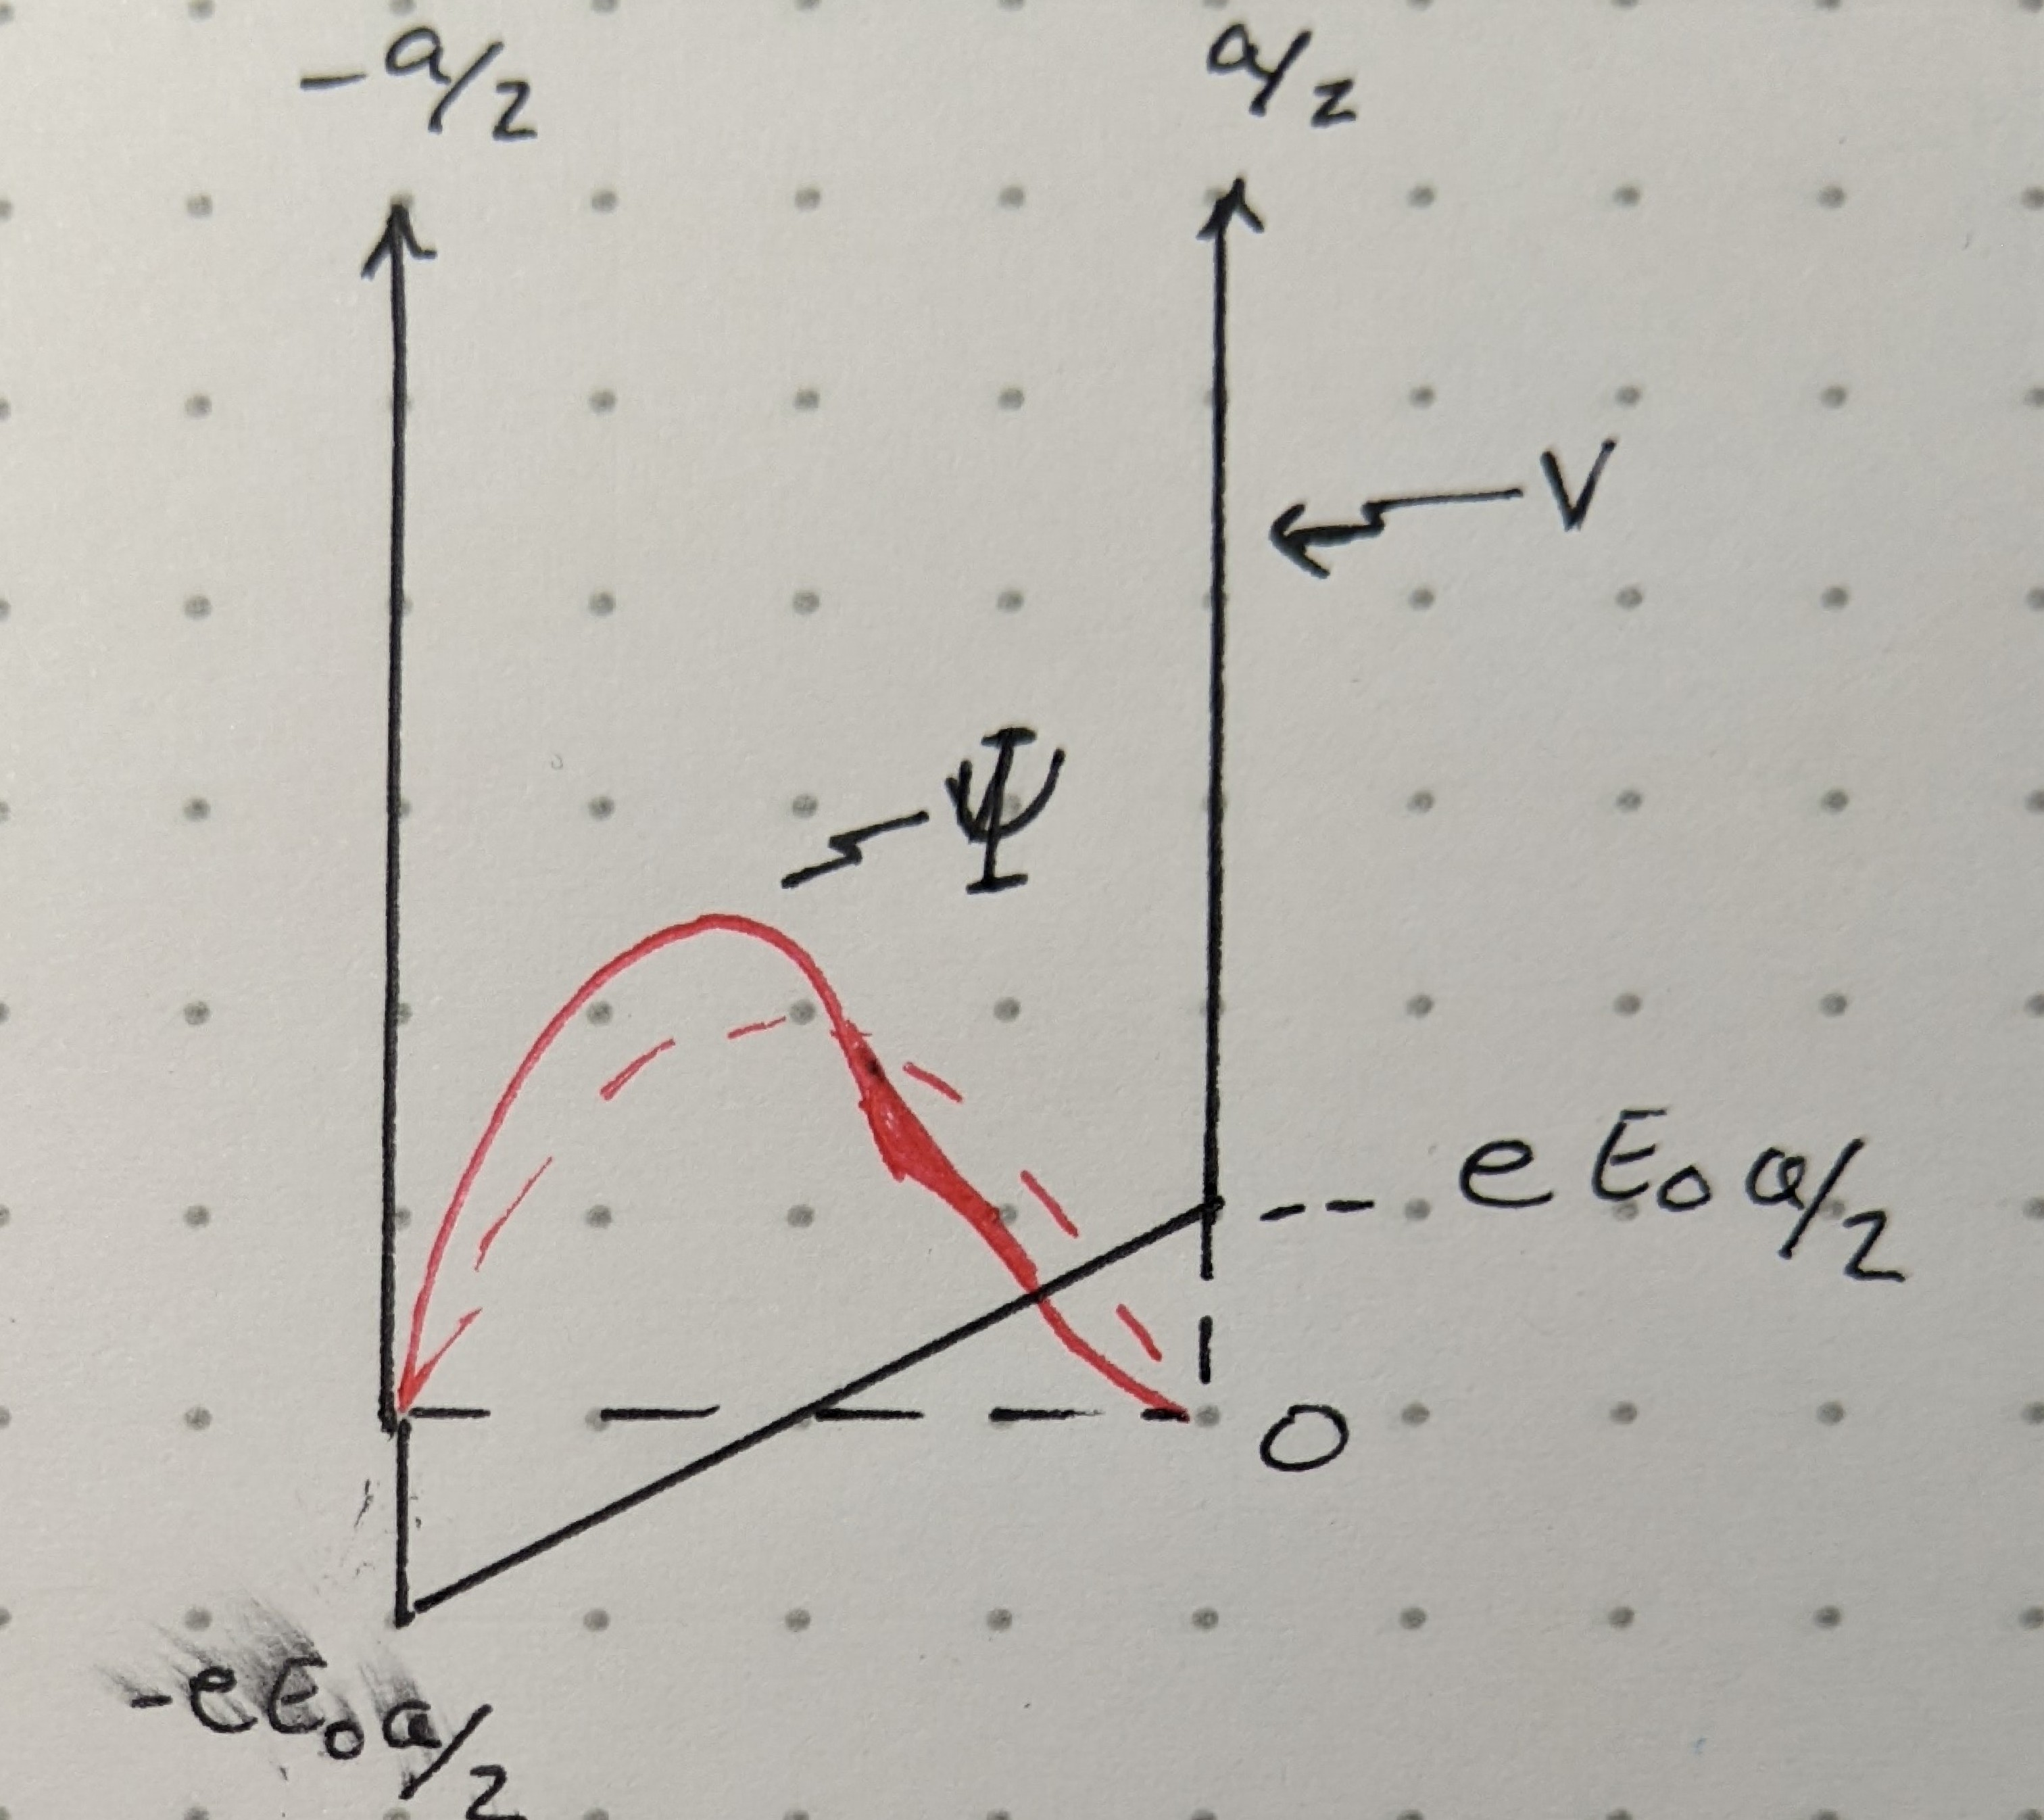
\includegraphics[width=0.5\textwidth]{phsx462_hw02_01.jpg}
	\caption{The image diagram for both part's {\bf a)} and {f)}. The dashed lines are the unperturbed system and the solid is the perturbed system.}
	\label{fig:5.1}
\end{figure}
\begin{enumerate}[label=\alph*)]
\item See Fig.~\ref{fig:5.1}
\item Let's start with the unperturbed system:
\begin{align*}
\ket{\Psi_n^0} & \rightarrow \sqrt{\frac{2}{a}}\sin(\frac{n\pi}{a}x + \frac{n\pi}{2}) & E_n & = \frac{\pi^2 \hbar^2 n^2}{a^2 2 m}
\end{align*}

Now, let's find the first solution.
\begin{flalign*}
E_n^{(1)} &= \ev{H^1}{\Psi_n^0} & \\
&= \int_{-a/2}^{a/2}\frac{2}{a}\sin[2](\frac{n\pi}{a}x + \frac{n\pi}{2})eE_0 \dd{x}&\\
&= \frac{2}{a}eE_0 \int_{-a/2}^{a/2} \left[\frac{1-\cos(\frac{2n\pi}{a}x + n\pi)}{2}\right]x\dd{x}&\\
&=\frac{1}{a}eE_0 \int_{-a/2}^{a/2}x - \cos(\frac{2n\pi}{a}x + n\pi)x\dd{x}&\\
&= \frac{1}{a}eE_0\left[0 - \left(\frac{a}{2n\pi}\sin(\frac{2n\pi}{a}x + n\pi)\right)x\eval_{-a/2}^{a/2} - \int_{-a/2}^{a/2}\frac{a}{2n\pi}\sin(\frac{2n\pi}{a}x + n\pi)\dd{x}\right]&\\
& = \frac{1}{a}eE_0\left[-\left(\frac{a}{2n\pi}\right)^2\cos(\frac{2n\pi}{a}x + n\pi)\eval_{-a/2}^{a/2}\right] = 0 \qquad \checkmark
\end{flalign*}

\item We need to invoke the second order approximation to the energy:
\[E_n^{(2)} = \sum_{m\neq n} \frac{\left|\mel{\Psi_m^0}{H_1}{\Psi_n^0}\right|^2}{E_n^0 - E_m^0}\]

First looking at the numerator:
\begin{flalign*}
\mel{\Psi_m^0}{H_1}{\Psi_n^0} &= \frac{2}{a}\int_{-a/2}^{a/2}\sin(\frac{m\pi}{a}x + \frac{m\pi}{2})eE_0 \, x \sin(\frac{n\pi}{a}x + \frac{n\pi}{2})\dd{x}&\\
& \text{ Through some IBP and actually pretty fun algebra:}&\\
& = eE_0\frac{a}{\pi^2}\left[\frac{\cos((m-n)\pi)}{(m-n)^2} - \frac{\cos((m+n)\pi)}{(m+n)^2} - \frac{1}{(m-n)^2} + \frac{1}{(m+n)^2}\right]&\\
& \text{ Setting }m=2 \text{ and } n=1 &\\
& \longrightarrow eE_0\frac{a}{\pi^2}\left[\frac{\cos(\pi)}{1^2} - \frac{\cos(3\pi)}{3^2} - \frac{1}{1^2} + \frac{1}{3^2}\right]&\\
& = eE_0\frac{a}{\pi^2}\left[-1 + \frac{1}{9} - 1 + \frac{1}{9}\right]&\\
& = -eE_0\frac{a}{\pi^2}\frac{16}{9}
\end{flalign*}

Dealing with the denominator:
\begin{flalign*}
\left(E_n^0 - E_m^0\right) &\rightarrow \left(E_1^0 - E_2^0\right) &\\
& = \frac{\pi^2 \hbar^2}{a^2 2m} - \frac{\pi^2 \hbar^2 4}{a^2 2m}&\\
& = \frac{\pi^2 \hbar^2}{a^2m}\left[\frac{1}{2} - \frac{4}{2}\right]&\\
& = \frac{3\pi^2 \hbar^2 }{2a^2 m}
\end{flalign*}

Putting both of these together:
\begin{flalign*}
E_n^{(2)} &= \left(-eE_0\frac{a}{\pi^2}\frac{16}{9}\right)\frac{3\pi^2 \hbar^2 }{2a^2 m}&\\
& = -\frac{a^4}{\pi^6}\frac{2^9}{3^5} \frac{m}{\hbar^2} &\\
& \boxed{= -24 \left(\frac{2}{3\pi}\right)^6 \frac{e^2 a^4 m}{\hbar^2}\left(E_0\right)^2} \qquad \checkmark
\end{flalign*}

\item To find the largest term in the $E_2^{(2)}$ we can just recognize that
\[\left|\mel{\Psi_m^0}{H_1}{\Psi_n^0}\right|^2 = \left|\mel{\Psi_n^0}{H_1}{\Psi_m^0}\right|^2\]
So, the numerator of the previous calculation can just be reused. The denominator will just gain a negative. So:
\[\boxed{E_2^{(2)}= 24 \left(\frac{2}{3\pi}\right)^6 \frac{e^2 a^4 m}{\hbar^2}\left(E_0\right)^2}\]

\item 
\begin{flalign*}
\Delta E = E_2 - E_1 & = \frac{\pi^2 \hbar^2 4}{a^2 2m} + 24 \left(\frac{2}{3\pi}\right)^6 \frac{e^2 a^4 m}{\hbar^2}\left(E_0\right)^2 - \frac{\pi^2 \hbar^2}{a^2 2m} + 24 \left(\frac{2}{3\pi}\right)^6 \frac{e^2 a^4 m}{\hbar^2}\left(E_0\right)^2 &\\
& \boxed{= \frac{3\pi^2 \hbar^2}{2a^2 m} + 48 \left(\frac{2}{3\pi}\right)^6 \frac{e^2 a^4 m}{\hbar^2}\left(E_0\right)^2}
\end{flalign*}

\item See Fig.~\ref{fig:5.1}

\end{enumerate}

\end{document}
